\subsection{Adaptacion del modelo Cinematico}
Como ya anticipamos, para este trabajo practico utilizaremos un robot omidireccional. Este cuenta con cuatro ruedas Mecanum dispuestas a los cuatro costados del robot, las cuales cuentan con rodillos especiales que permiten transmitir parte de la fuerza en direccion de un angulo definido.
%motivacion -> para poder posicionarte

Como primer desafío buscaremos determinar la velocidad de los actuadores y la velocidad en cada uno de los ejes de livertad del robot. Para esto adaptaremos el modelo cinematico visto durante la materia para a este nuevo tipo de actuadores utilizando el paper provisto por la catedra, las formulas de cinematica directa pasarán a ser.


$$v_x(t)=(w_1+w_2+w_3+w_4).r/4$$
$$v_y(t)=(-w_1+w_2+w_3-w_4).r/4$$
$$w_z(t)=(-w_1+w_2-w_3+w_4).r/(4(l_x+l_y))$$


Y las de cinematica inversa:

$$ w_1 = 1/r (v_x - v_y - (l_x + l_y)w_z$$
$$ w_2 = 1/r (v_x + v_y + (l_x + l_y)w_z$$
$$ w_3 = 1/r (v_x + v_y - (l_x + l_y)w_z$$
$$ w_4 = 1/r (v_x - v_y + (l_x + l_y)w_z$$

%se podria hacer una lista.
Donde $v_x$, $v_y$ y $w_z$ son las velocidades lineares y angular del robot, $r$ el radio de las ruedas (asumiremos que todas las ruedas tienen exactamente el mismo radio), $l_x$ la mita de la distancia entre las dos ruedas delanteras y $l_y$ la mitad de la distancia entre una rueda delantera y una rueda tracera.
$w_1,w_2,w_3,w_4$ las velocidades angulares de las cuatro ruedas.

En particular para nuestro robot, tomaremos $r =0.05 $ metros, $l_x = l_y = 0.175 $ metros.

\subsubsection{Experimentación}

En este apartado buscaremos validar que el moldeo antes descripto se condice con la realidad. Para ello, enviaremos mensajes a travez de rostopic con comandos de velocidad lineal y esperaremos ver que el modelo sepa traducir y aplicar la velocidad deseada en los actuadores. Luego utilizando los mensajes de cinematica inversa esperamos que el modelo pueda traducir nuevamente las velocidades angulares de los actuadores a las velocidades lineales y que estas se condigan con las que enviamos.

% Plantear experimentos que permitan validar y evaluar la efectividad
% del modelo. Entre los experimentos a realizar se deben incluir gr ́aficos de consignas de velocidades lineales y angular
% del robot junto a las correspondientes velocidades reales ejercidas por el robot, para su comparaci ́on. Asimismo, se
% debe incluir un gr ́
% afico que permita comparar la pose del robot estimada seg ́
% un odometr ́ıa con la real informada por el
% simulador.

\subsection{Adaptación del control a lazo cerrado}

Al igual que para el modelo diferencial queremos que el robot se pueda transladar de una posicion inicial $(x_i,y_i,w_i)$ a una posicion final $(x_f,y_f,w_f)$


En este caso, al tener un modelo cinematico holonómico las cuentas se simplifican con respecto al modelo diferencial: Al tener control independiente sobre cada velocidad puedo plantear, para cada dimención por separado:

$$v_x = x_f - x_i / (t_f - t_i)$$
$$v_y = y_f - y_i / (t_f - t_i)$$
$$v_x = w_f - w_i / (t_f - t_i)$$

\subsubsection{Experimentación}


\subsection{Modelado de EKF}
En el caso de un robot omidireccional, lo que cambia respecto al modelo diferencial usado previamente es que aumentan los grados de libertad posibles en la translación. Ahora es posible que el robot se mueva tanto en $x$ como en $y$ y $\theta$.

Por este motivo, el vector $\overrightarrow{u}$ que representa las entradas de contro cambia de la siguiente manera:

$$\overrightarrow{u} = \begin{bmatrix}
         Vx \\
         Vy \\
         w 
        \end{bmatrix}$$


El modeo de estado $\overrightarrow{x}$ se mantiene, ya que el robot permanece igual a la del modelo anterior:

$$\overrightarrow{x} = \begin{bmatrix}
         x \\
         y \\
         \theta 
        \end{bmatrix}$$

Dada la modificacón en $\overrightarrow{x}$, ahora el modelo de movimiento $f(\overrightarrow{x},\overrightarrow{u}, \overrightarrow{w})$ ahora pasará a ser:

$$f(\overrightarrow{x},\overrightarrow{u}, \overrightarrow{w})= \begin{bmatrix}
         x + Vx \Delta t cos(\theta) + Vy \Delta t sen(\theta) + w_1 \\
         y + Vx \Delta t sen(\theta) + Vy \Delta t cos(\theta) + w_2 \\
         norm_{[-\pi,\pi]} (\theta + w \Delta t) + w_3
         \end{bmatrix}$$

Calculando los jacobianos de la función $f$ respecto a $\overrightarrow{x}$ y a $\overrightarrow{w}$ respectivamente, tenemos:

$$A= \begin{bmatrix}
         1 & 0 & -sen(\theta)\Delta x + cos(\theta) \Delta t V y\\
         1 & 0 & -cos(\theta)\Delta x - sen(\theta) \Delta t V y \\
         0 & 0 & 1
         \end{bmatrix}$$

$$W$$

El modelo de sensado $h(\overrightarrow{x},\overrightarrow{v})$ y las mediciones $z$ al no depender del tipo de movimiento que el robot omnidireccional ejerce, no se ve afectado por el modelo omnidireccional asi que permanecen como vimos previamente en la materia. Luego, la matriz Jacobiana H tampoco se ve afectada con respecto a lo que visto.

%TODO: modificacion de la covarianza inicial.

\subsubsection{Experimentación}

En esta seccion buscamos experimentar que tan bueno resulta el modelo EKF con las modificaciones descriptas previamente.

Partiendo de un punto en el que el robot se encuentra frente a tres postes, podemos observar que logra estimar su posición con una matriz de covarianza (en azul) casi nula.

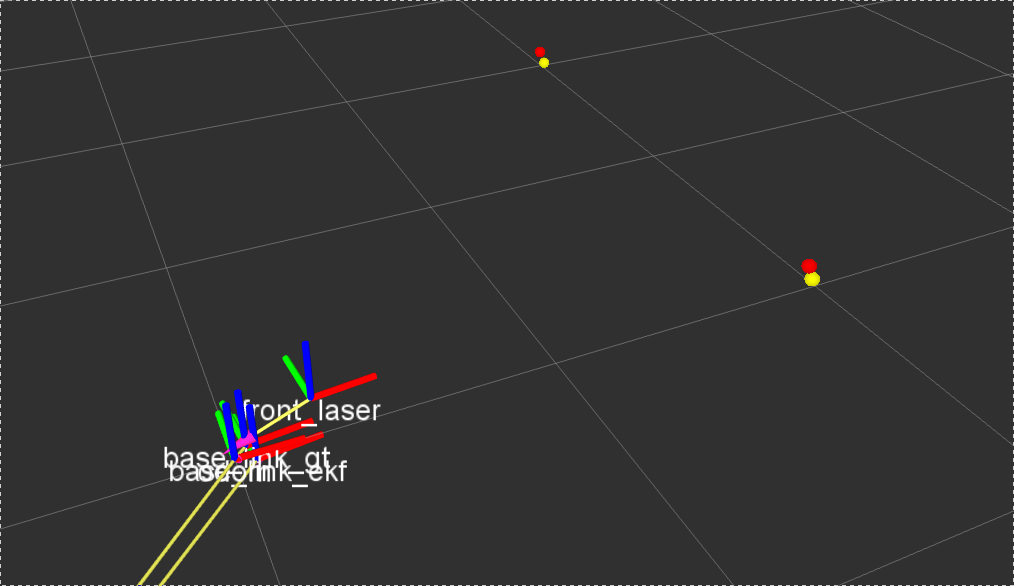
\includegraphics[scale=0.3]{punto4/ekfViendoTodosLosPostes.png}

Reduciendo la distancia entre los postes y el robot, logramos que este solo vea dos al mismo tiempo. En este momento su covarianza continua siendo casi imperceptible en la imagen.

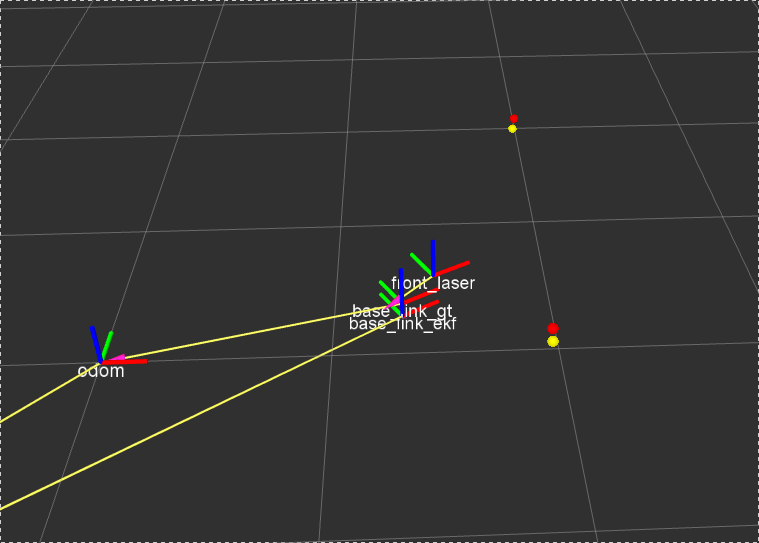
\includegraphics[scale=0.3]{punto4/ekfViendoDosPostes.png}

Ahora posicionando el robot para que solo cense un poste, el grado de certeza decae considerablemente. Dado que ahora solo tenemos la referencia al eje $x$ la covarianza en el eje $y$ empieza a aumentar.

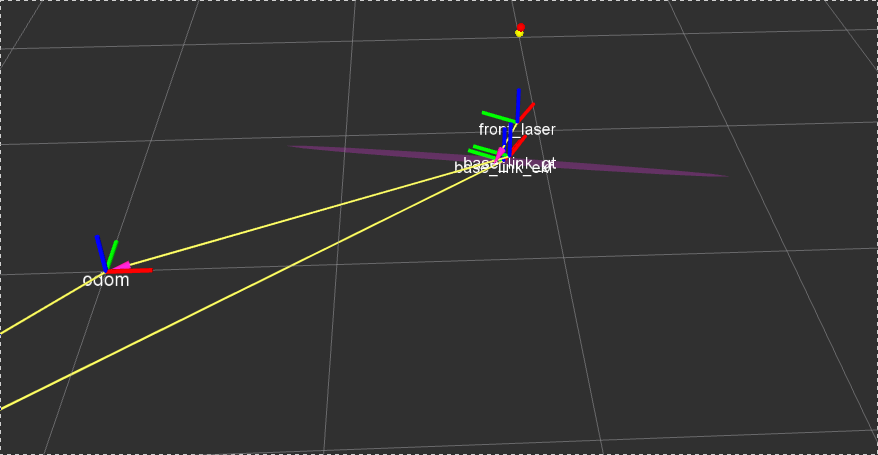
\includegraphics[scale=0.3]{punto4/ekfViendoUnPoste.png}

Si ahora volvemos a censar dos postes podemos observar como el robot tiene la posibilidad de recuperarse y volver a predecir su posicion de manera precisa, reduciendo la covarianza en el eje $y$.

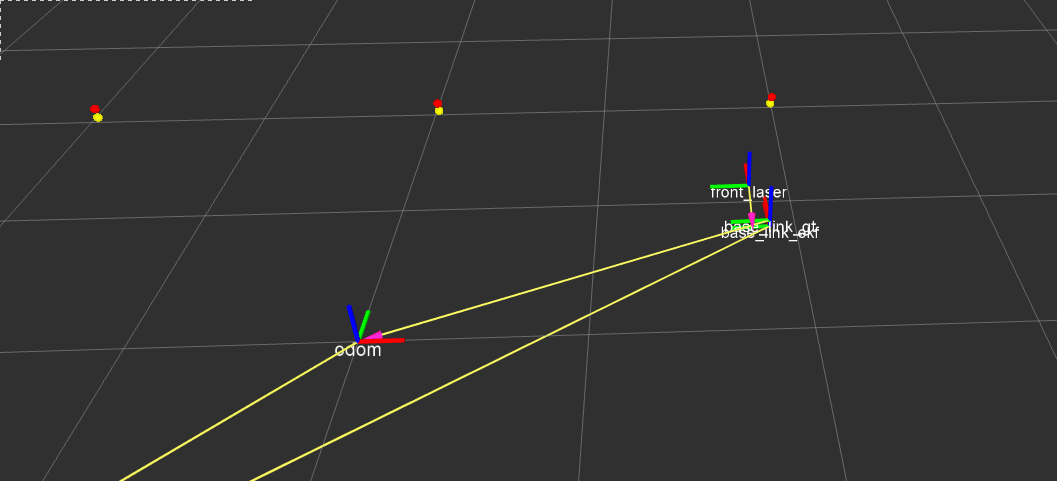
\includegraphics[scale=0.3]{punto4/ekfViendoTresPostesOtraVez.png}

finalmente, si el robot no es capaz de sensar ningun poste, la covarianza tanto en x como en y empiezan a aumentar.

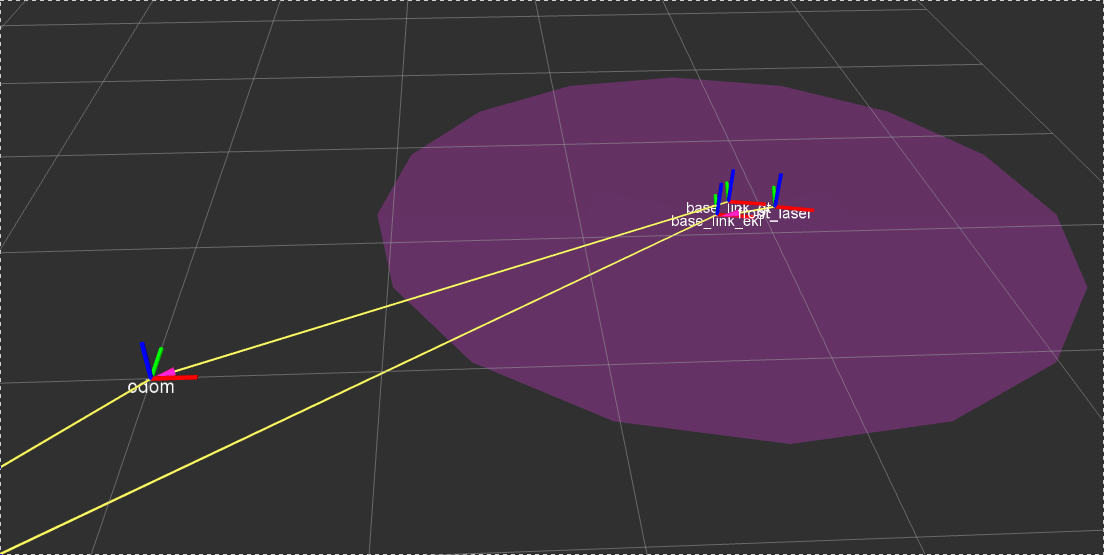
\includegraphics[scale=0.3]{punto4/ekfSinVerNingunPoste.png}

%conclucìón, EKF te permite darle mucho mas velocidad sin perder precición, en cambio con lazo cerrado, si aumentas mucho la cte, se te va todo al carajo.